\section{Results}
\label{sec:results}

\subsection{Prototype study and why early wins were large}
\label{sec:prototype}

The first quantitative pass ran in the client-side V1 stack against relatively weak replicas of Diviner-class temperature, radiation, dust, meteor, solar, and seismic products. Under that setup the mean skill across hazards favored LIPAS (Fig.~\ref{fig:proto}). Those early wins are not evidence that the locked hybrid beats mature agency models.

Three design choices drove the spread. First, the client V1 model and scoring path differ from the locked train-2 blend in Eq.~\eqref{eq:blend}. Second, several replica baselines were thin proxies rather than full operational models, so the comparison favored the integrated client. Third, some hazard scores used circular or proxy targets, which inflate apparent skill without independent surface truth. The prototype is therefore treated as an engineering checkpoint only. The locked windows below replace it for accuracy claims.

\begin{figure}[t]
\centering
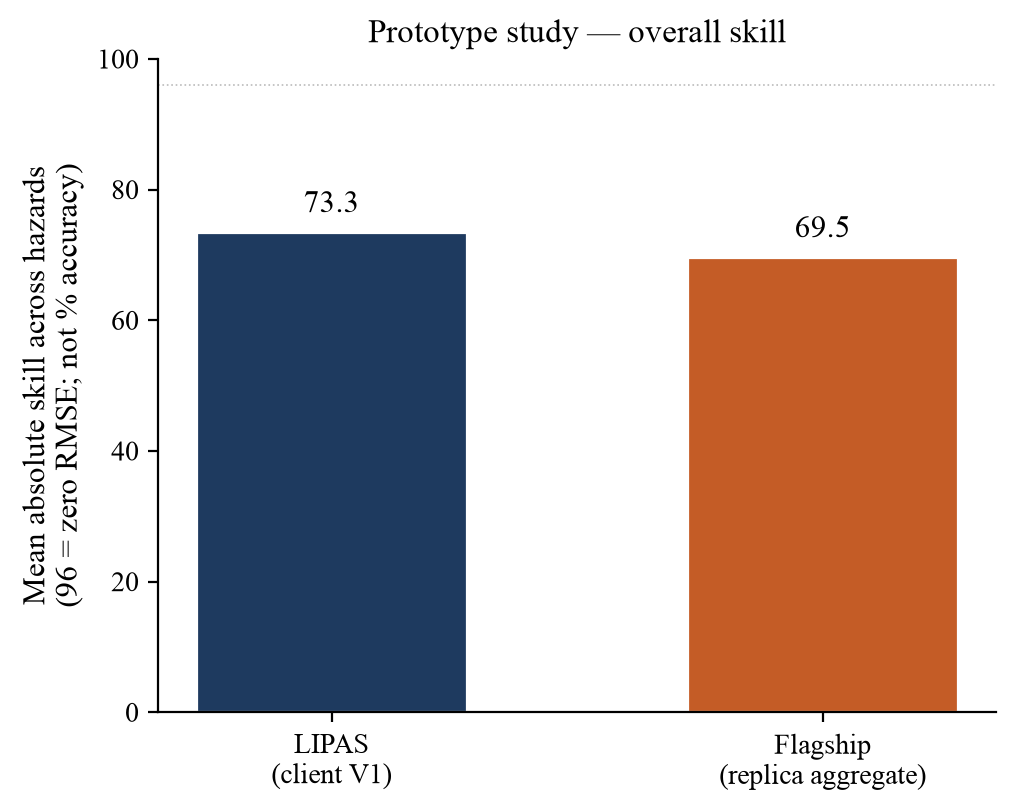
\includegraphics[width=0.72\linewidth]{fig_prototype_lipas_vs_flagship.png}
\caption{Prototype study mean skill: LIPAS (client V1) versus a single flagship-replica aggregate. Two bars only, same within-hazard skill definition as Windows~A and~B. The early lead reflects weak replicas and a different model/scoring path, not the locked train-2 result.}
\label{fig:proto}
\end{figure}

\subsection{LIPAS versus Diviner-class temperature (prototype path)}
\label{sec:diviner}

Figure~\ref{fig:diviner} shows an early daytime temperature comparison at $(0^\circ\mathrm{N},\ 0^\circ\mathrm{E})$ before temperature was locked to the physics path. The early client overshoots the Diviner-class reference and the observed proxy near peak heating. That failure is part of why the locked blend sets temperature weight to zero and why Windows~A and~B report temperature as a physics tie rather than an ML win. The figure belongs to the prototype evaluation era. After this checkpoint the paper moves to the locked studies.

\begin{figure}[t]
\centering
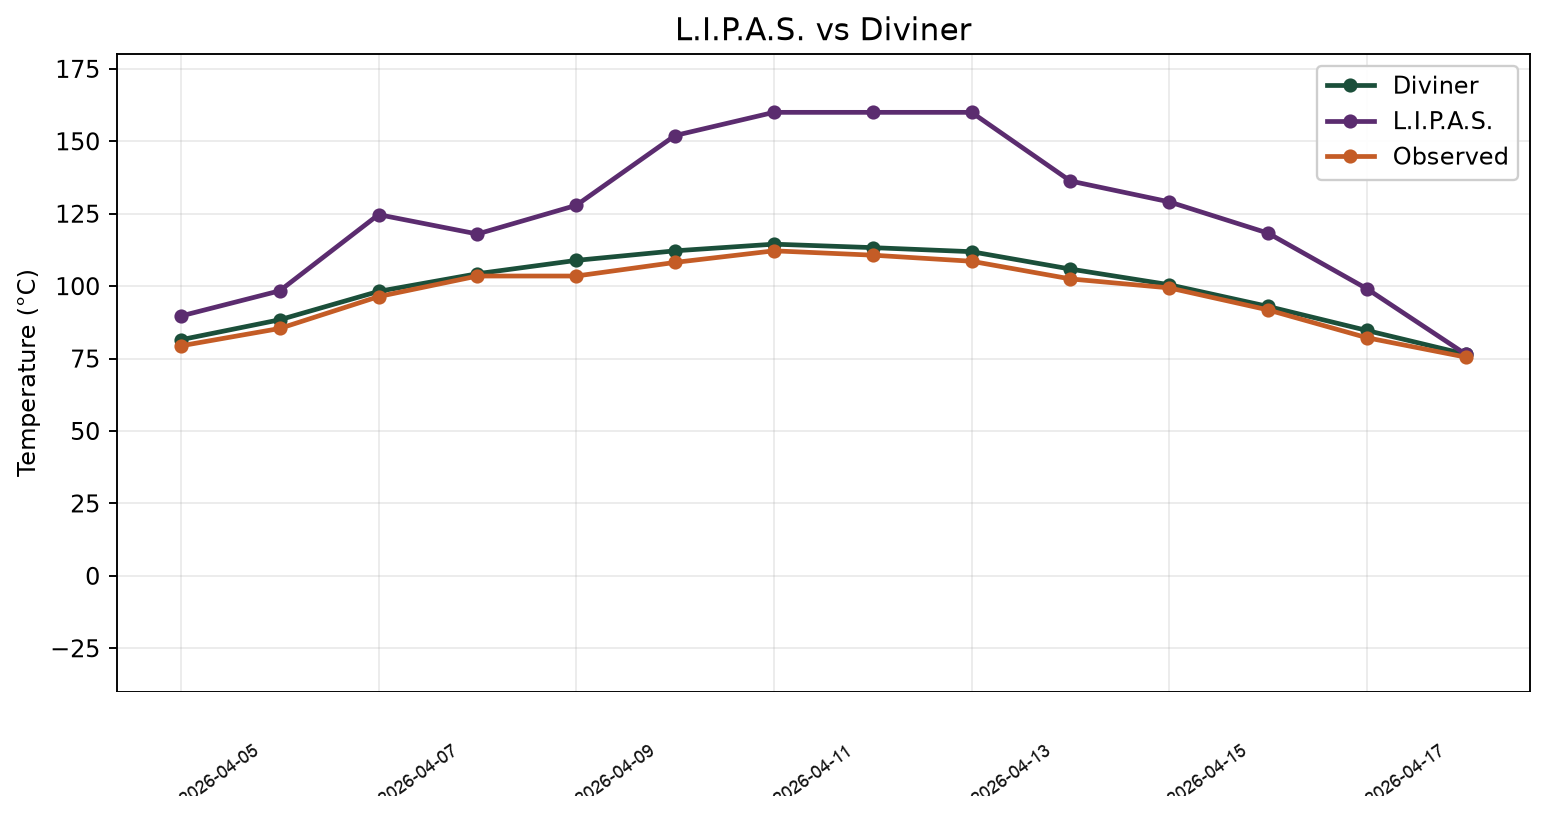
\includegraphics[width=0.92\linewidth]{fig_lipas_vs_diviner.png}
\caption{LIPAS versus Diviner-class temperature reference on the prototype daytime path at $0^\circ\mathrm{N}$, $0^\circ\mathrm{E}$. Early client temperature overshoots the reference near peak heating. Prototype-era figure; locked windows use physics-led temperature under blend weight zero.}
\label{fig:diviner}
\end{figure}

\noindent\textit{Reading Fig.~\ref{fig:diviner} for the prototype study.} The temperature channel did not ``win'' in this early plot. Combined with weak replicas on other channels, that mix is exactly why a single mean-skill bar can still look favorable in Fig.~\ref{fig:proto} while individual physics channels remain untrustworthy. The later locked studies therefore emphasize solar and radiation RMSE, where the replica comparison is more informative, and treat temperature as a shared physics path.

\subsection{Locked Window A (night-dominant)}
\label{sec:windowA}

Window~A uses the locked blend. Solar activity improves relative to the replica (RMSE 4.10 versus 4.66). Radiation does not: night-dominant RMSE is 0.119 for LIPAS versus 0.102 for the replica. Temperature, moonquakes, and dust remain physics ties. Micrometeorite skill is circular under blend weight zero and is not treated as an independent win.

\begin{figure}[t]
\centering
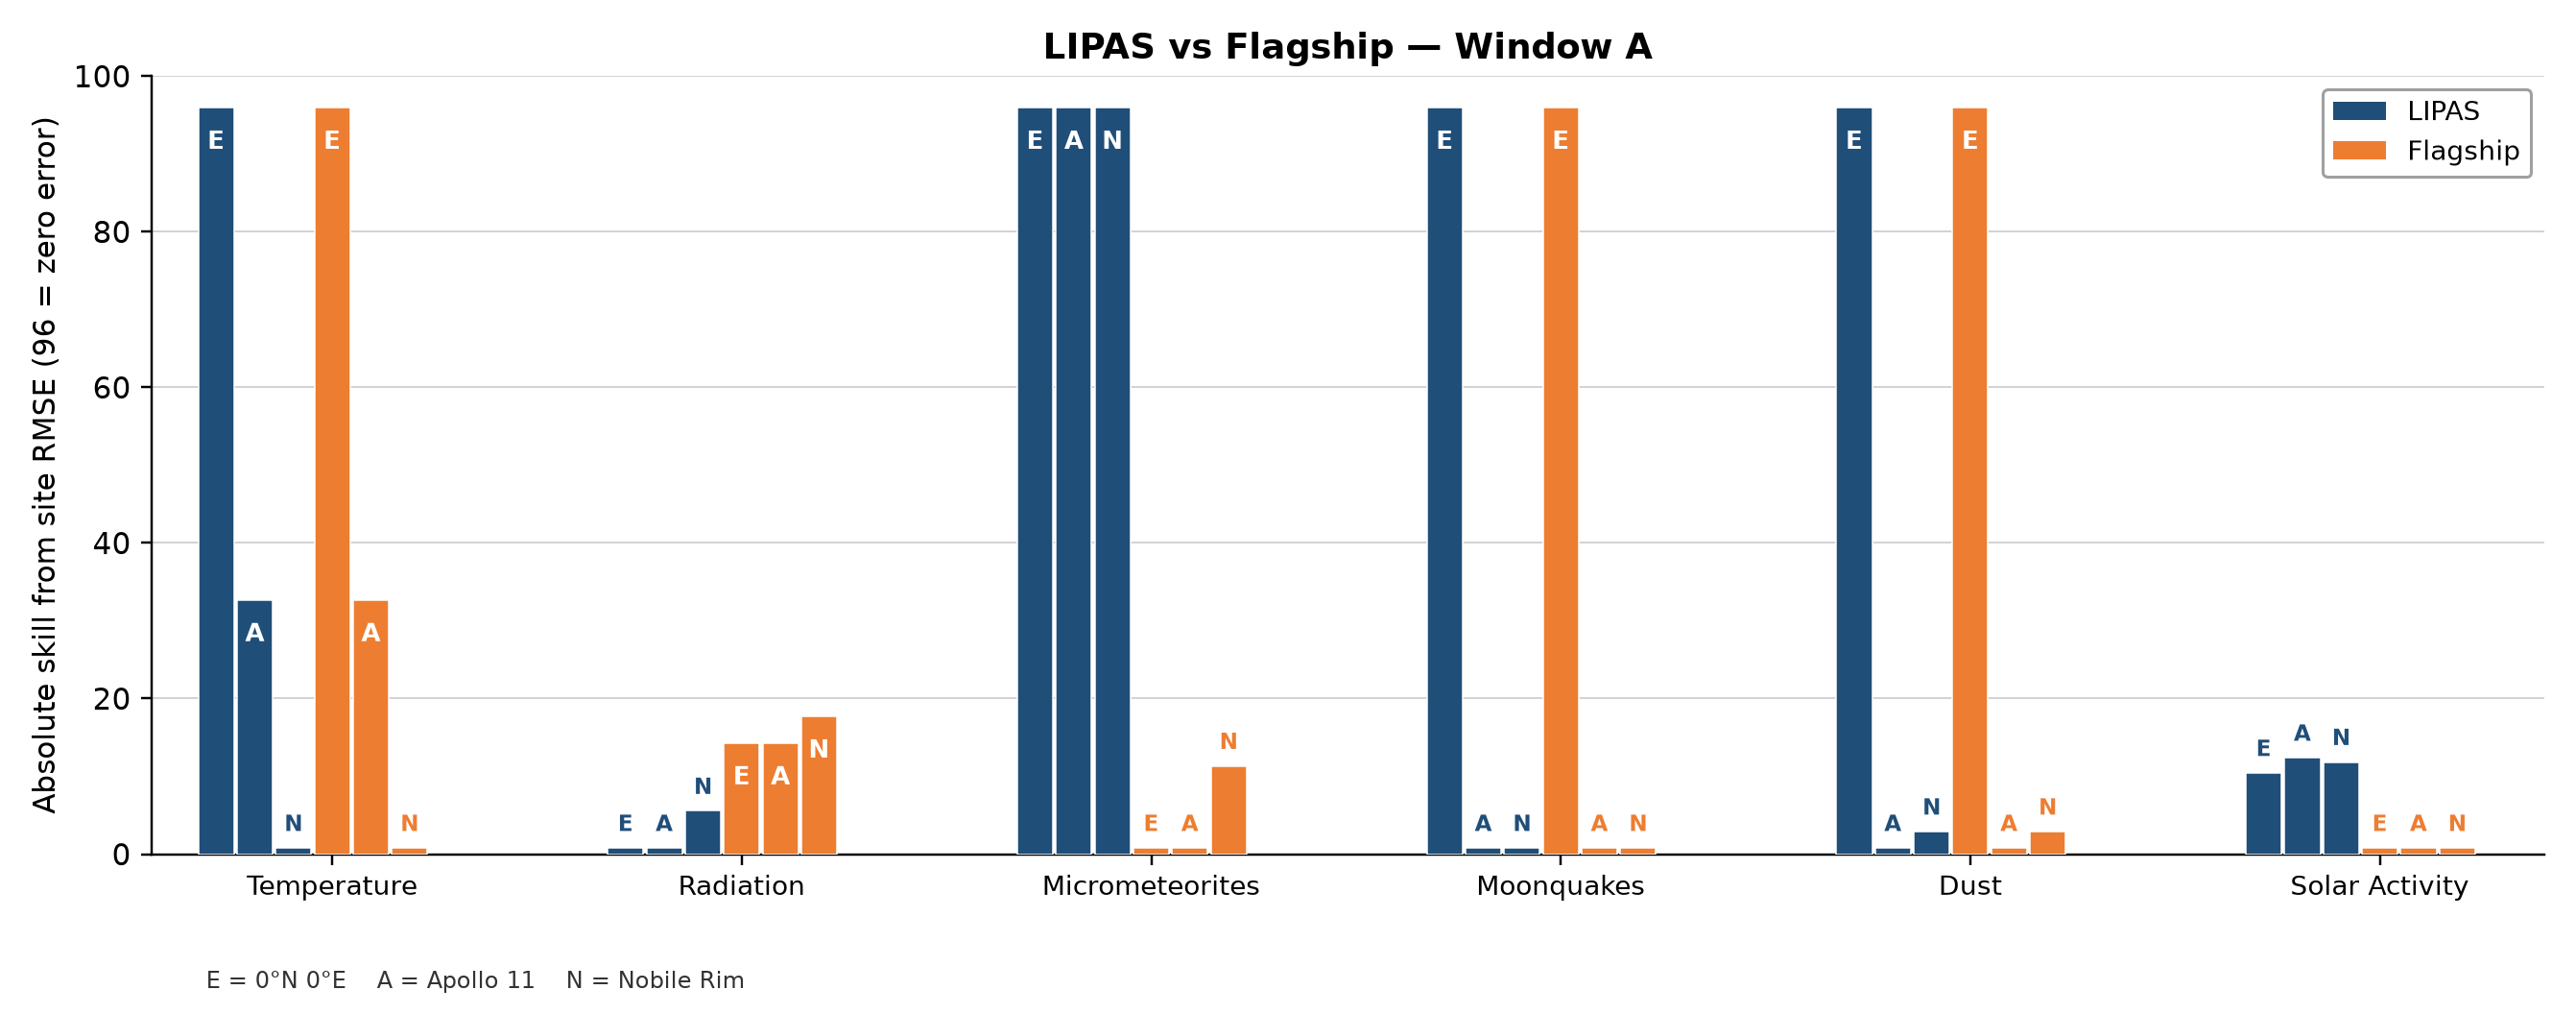
\includegraphics[width=0.95\linewidth]{fig_windowA_skill.png}
\caption{Window~A locked skill by hazard and site. Within-hazard skill only; no cross-hazard height equalization. Location key: E = $0^\circ\mathrm{N}$, $0^\circ\mathrm{E}$; A = Apollo~11; N = Nobile Rim.}
\label{fig:wa}
\end{figure}

\subsection{Locked Window B (dayside quiet)}
\label{sec:windowB}

Window~B again shows a solar gain (RMSE 4.99 versus 5.99) while radiation remains worse than the replica under quiet dayside conditions (0.0188 versus 0.00266). Physics ties and circular micrometeorite scoring match Window~A.

\begin{figure}[t]
\centering
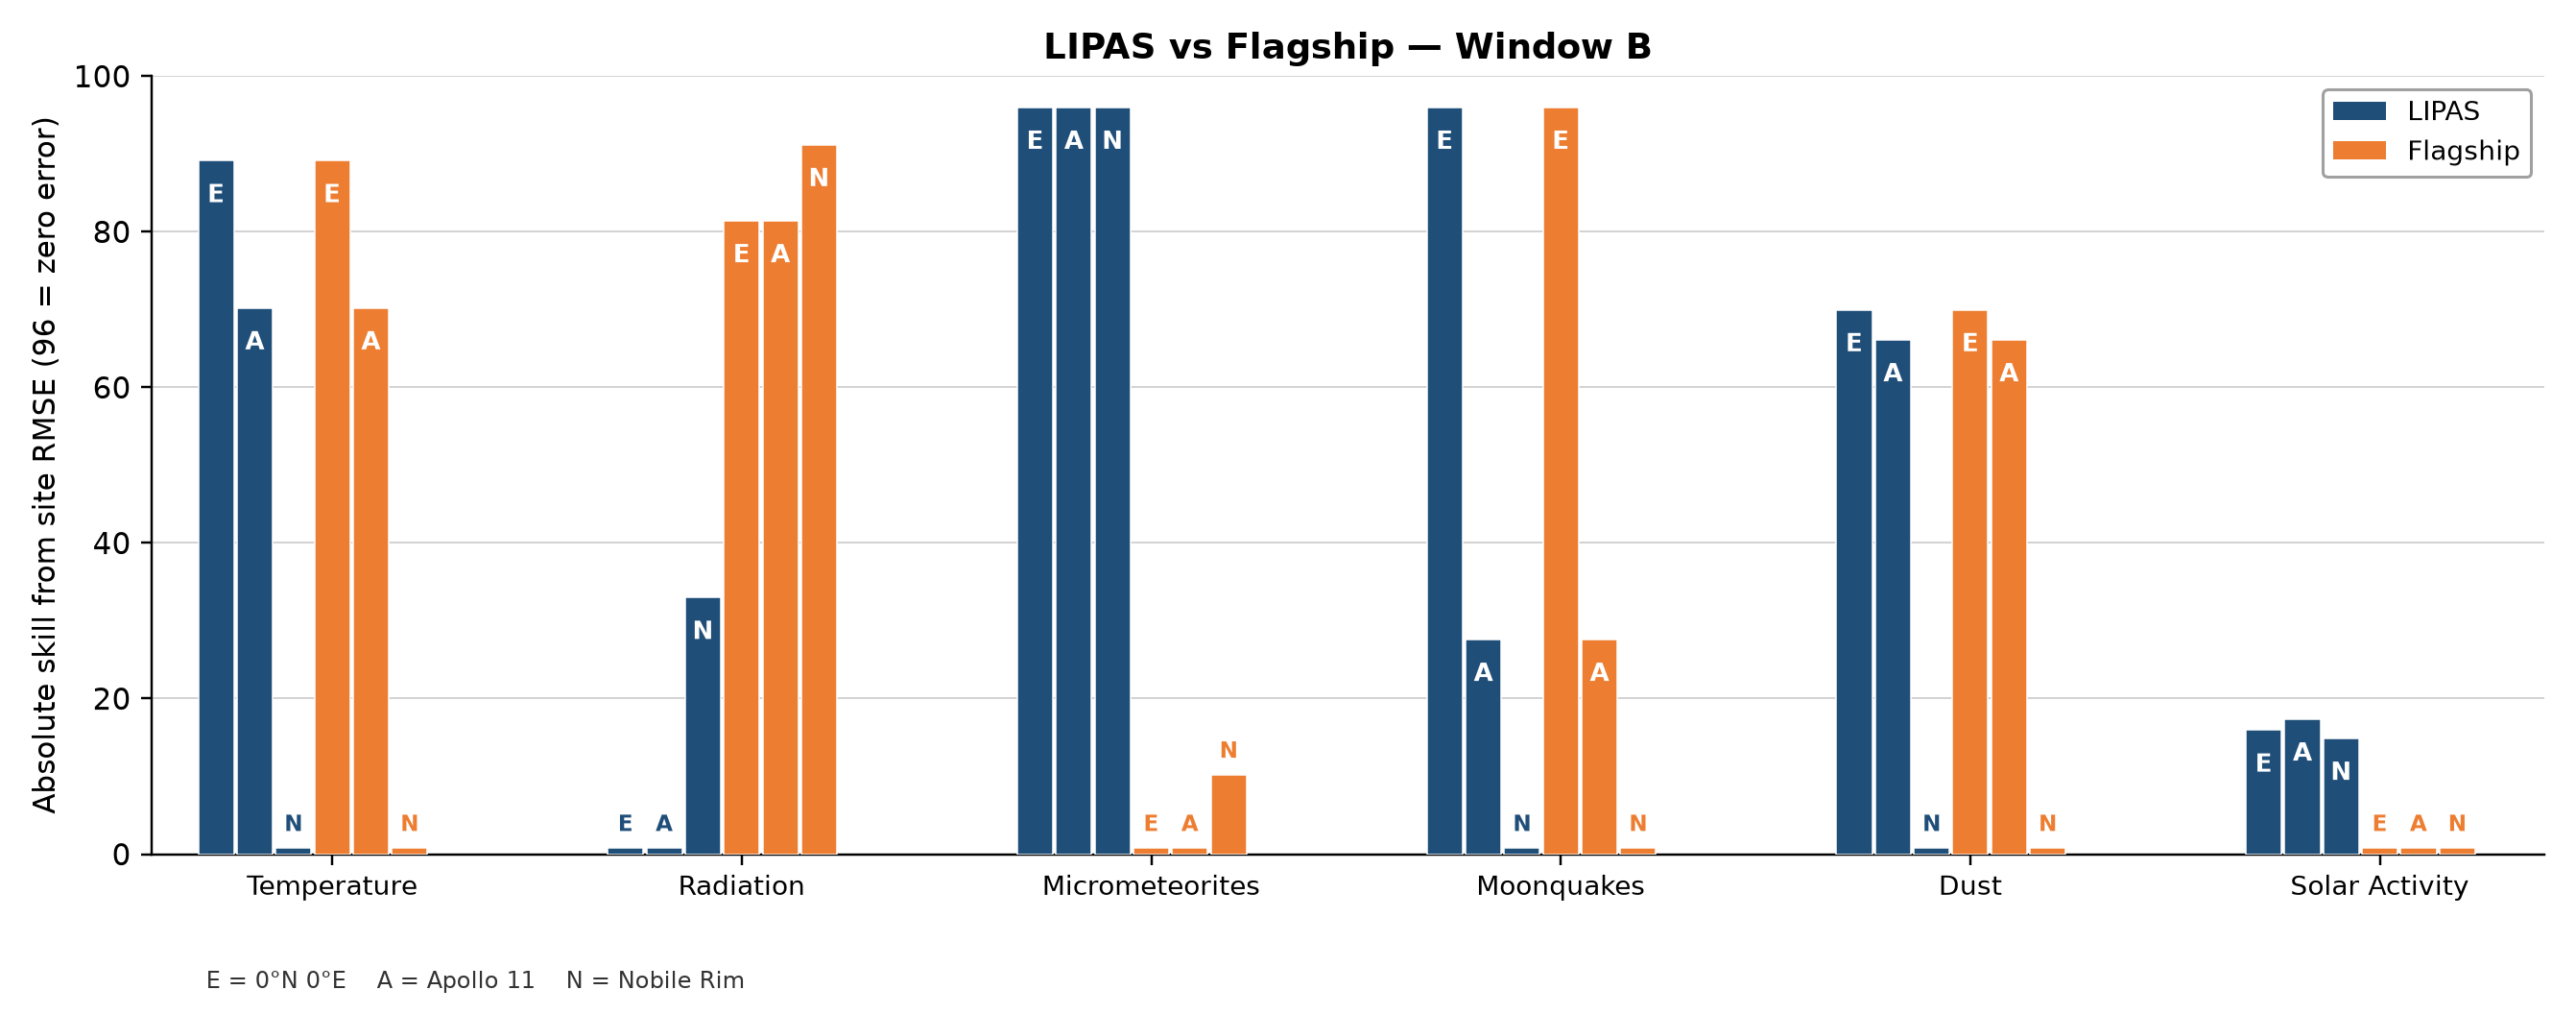
\includegraphics[width=0.95\linewidth]{fig_windowB_skill.png}
\caption{Window~B locked skill by hazard and site. Same blend and replica stack as Window~A. Location key as in Fig.~\ref{fig:wa}.}
\label{fig:wb}
\end{figure}

\subsection{Qualitative comparison}
\label{sec:qual}

A structured qualitative framework scores nine criteria (coverage, fusion, forecasting, spatial reach, real-time operations, robustness, validation, usability, openness) against DONKI, Diviner, LDEX, Apollo PSE, MEM~3, and GOES-18 (full rubric and references in Appendix~B). LIPAS ranks high on multi-hazard coverage, fusion, and dashboard usability: one interface exposes six hazards and selectable lunar coordinates. Validation and robustness are only moderate because continuous co-located surface truth is missing for several hazards and because many scores rely on proxies. Specialized agency products invert that pattern: high validation inside one domain, low multi-hazard coverage.

For the research questions this means: RQ2 is supported on usability and coverage; RQ3 is only partly supported and must rest on the locked windows, not on the prototype bars; RQ1 is supported as a working hybrid architecture but not as a claim of uniform accuracy gains. Deeper interpretation of trade-offs is taken up in Section~\ref{sec:discussion}.

\subsection{Mission simulation}
\label{sec:mission}

A short mission timeline overlays caution and no-go markers for planning context (Fig.~\ref{fig:mission}). Legend markers use red for all compared paths so the timeline reads cleanly in print. This study is operational illustration, not a substitute for the locked RMSE tables.

\begin{figure}[t]
\centering
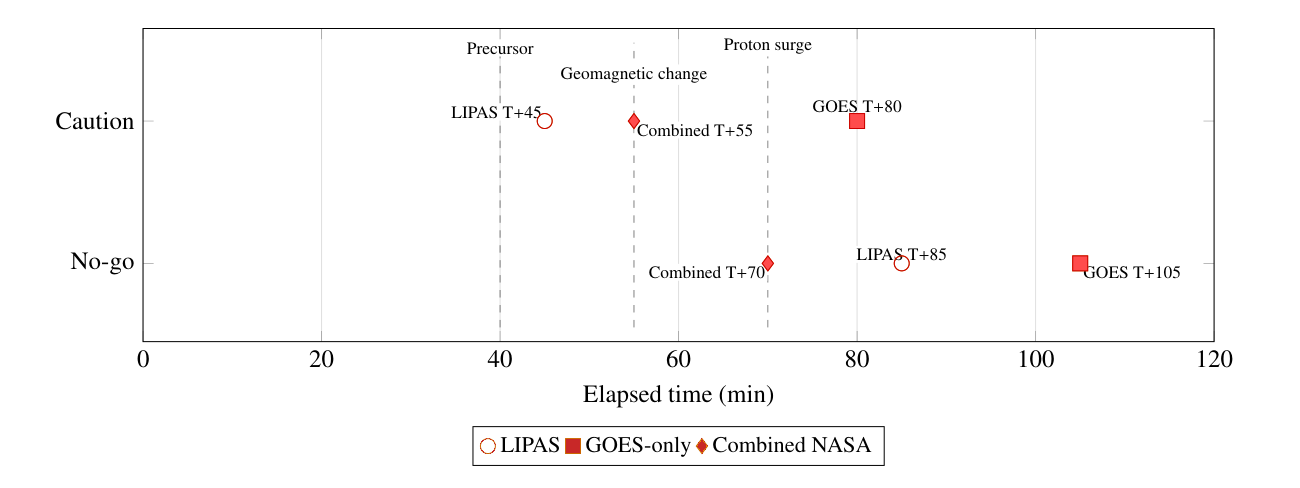
\includegraphics[width=0.95\linewidth]{fig_mission_timeline.png}
\caption{Mission simulation timeline with caution and no-go markers. Legend uses red markers for LIPAS, GOES-only, and Combined NASA paths. Operational context only.}
\label{fig:mission}
\end{figure}

\subsection{Ablation}
\label{sec:ablation}

Hazard-weight ablation shows that nonzero machine-learning weight on solar activity and radiation changes residuals as expected under Eq.~\eqref{eq:blend}, while zero-weight hazards stay on their physics or proxy paths. Ablation supports sensitivity interpretation; it does not create new locked wins.